% !TeX root = RJwrapper.tex
\title{Teaching Computers to See Patterns in Scatterplots with
Scagnostics}
\author{by Harriet Mason, Stuart Lee, Ursula Laa, and Dianne Cook}

\maketitle

\abstract{%
An abstract of less than 150 words.
}

\hypertarget{introduction}{%
\section{Introduction}\label{introduction}}

Visualising high dimensional data is often difficult and requires a
trade-off between the usefulness of the plots and maintaining the
structures of the original data. Scagnostics (scatterplot diagnostics)
are a set of visual features that can be used to identify interesting
and abnormal scatterplots, and thus give a sense of priority to the
variables we choose to visualise. This proposal will discuss the
creation of an R package that will provide a user-friendly method to
calculate these scagnostics. The package will be tested on datasets with
known interesting visual features to ensure the scagnostics are working
as expected, before finally being used to explore and describe a time
series dataset.

As the number of dimensions in a dataset increases, the process of
visualising its structure and variable dependencies becomes more
tedious. This is because the number of possible pairwise plots rises
exponentially with the number of dimensions. Datasets like Anscombe's
quartet \citep{anscombe} or the datasaurus dozen \citep{datasaurpkg}
have been constructed such that each pairwise plot has the same summary
statistics but strikingly different visual features. This design is to
illustrate the pitfalls of numerical summaries and the importance of
visualisation. This means that despite the issues that come with
increasing dimensionality, visualisation of the data cannot be ignored.
Scagnostics offer one possible solution to this issue.

The term scagnostics was introduced by John Tukey in 1982 \citep{tukey}.
Tukey discusses the value of a cognostic (a diagnostic that should be
interpreted by a computer rather than a human) to filter out
uninteresting visualisations. He denotes a cognostic that is specific to
scatter plots a scagnostic. Up to a moderate number of variables, a
scatter plot matrix (SPLOM) can be used to create pairwise
visualisations, however, this solution quickly becomes infeasible. Thus,
instead of trying to view every possible variable combination, the
workload is reduced by calculating a series of visual features, and only
presenting the outlier scatter plots on these feature combinations.

There is a large amount of research into visualising high dimensional
data, most of which focuses on some form of dimension reduction. This
can be done by creating a hierarchy of potential variables, performing a
transformation of the variables, or some combination of the two.
Unfortunately none of these methods are without pitfalls. Linear
transformations are subject to crowding, where low level projections
concentrate data in the centre of the distribution, making it difficult
to differentiate data points \citep{crowding}. Non-linear
transformations often have complex parameterisations, and can break the
underlying global structure of the data, creating misleading
visualisations. While there are solutions within these methods to fix
these issues such as a burning sage tour for crowding
\citep{burningsage} or liminal package for maintaining global structure
\citep{liminal} all these methods still involve some transformation of
the data. Scagnostics gives the benefit of allowing the user to view
relationships between the variables in their raw form. This means they
are not subject to the linear transformation issue of crowding, or the
non-linear transformation issue of misleading global structures. That
being said, only viewing pairwise plots can leave our variable
interpretations without context. Methods such as those shown in
\emph{ScagExplorer} \citep{scagexplorer} try to address this by
visualising the pairwise plots in relation to the scagnostic measures
distribution, but ultimately the lack of context remains one of the
limitations of using scagnostics alone as a dimension reduction
technique.

Scagnostics are not only useful in isolation, they can be applied in
conjunction with other techniques to find interesting feature
combinations of the transformed variables. The tourr projection pursuit
currently uses a selection of scagnostics to identify interesting low
level projections and move the visualisation towards them
\citep{tourrpp}. Since scagnostics are not dependent on the type of
data, they can also be used to compare and contrast scatter plots
regardless of the discipline. In this way, they are a useful metric for
something like the comparisons described in \emph{A self-organizing,
living library of time-series data}, which tries to organise time series
by their features instead of on their metadata \citep{sots}.

Several scagnostics have been previously defined in
\emph{Graph-Theoretic Scagnostics} \citep{scag}, which are typically
considered the basis of the visual features. They were all constructed
to range {[}0,1{]}, and later scagnostics have maintained this scale.
The formula for these measures were revised in \emph{Scagnostic
Distributions} and are still calculated according to this paper
\citep{scagdist}. In addition to the main nine, the benefit of using two
additional association scagnostics were discussed in Katrin Grimm's PhD
thesis \citep{Grimm}. These two association measures are also used in
the tourr projection pursuit \citep{tourrpp}.

There are two existing scagnostics packages, \emph{scagnostics}
\citep{scagdist} and the archived package \emph{binostics}
\citep{binostics}. Both are based on the original C++ code from
\emph{Scagnostic Distributions} \citep{something}, which is difficult to
read and difficult to debug. Thus there is a need for a new
implementation that enables better diagnosis of the scagnostics, and
better graphical tools for examining the results.

This paper describes the R package, \texttt{cassowaryr} that computes
the currently existing scagnostics, and adds several new measures. The
paper is organised as follows. The next section explains the
scagnostics. This is followed by a description of the implementation.
Several examples using collections of time series and XXX illustrate the
usage.

\hypertarget{scagnostics}{%
\section{Scagnostics}\label{scagnostics}}

\hypertarget{building-blocks-for-the-graph-based-metrics}{%
\subsection{Building blocks for the graph-based
metrics}\label{building-blocks-for-the-graph-based-metrics}}

In order to capture the visual structure of the data, graph theory is
used to calculate most of the scagnostics. The pairwise scatter plot is
re-constructed as a graph with the data points as vertices and the edges
are calculated using Delaunay triangulation. In the package this
calculation is done using the alphahull package \citep{alphahull} to
construct an object called a scree. This is the basis for all the other
objects that are used to calculate the scagnostics (except for
monotonic, dcor and splines which use the raw data). The graph (screen
object) is then used to construct the three key structures on which the
scagnostics are based; the convex hull, alpha hull and minimum-spanning
tree (MST).

\begin{itemize}
\item
  \textbf{Convex hull:} The outside vertices of the graph, connected to
  make a convex polygon that contains all points. It is constructed
  usnig the tripack package.
\item
  \textbf{Alpha hull:} A collection of boundaries that contain all the
  points in the graph. Unlike the convex hull, it does not need to be
  convex. It is calculated using the alphahull package
  \citep{alphahull}.
\item
  \textbf{MST:} the minimum spanning tree, i.e the smallest distance of
  branches that can be used to connect all the points. In the package it
  is calculated from the graph using the igraph package \citep{igraph}.
\end{itemize}

\begin{Schunk}
\begin{figure}
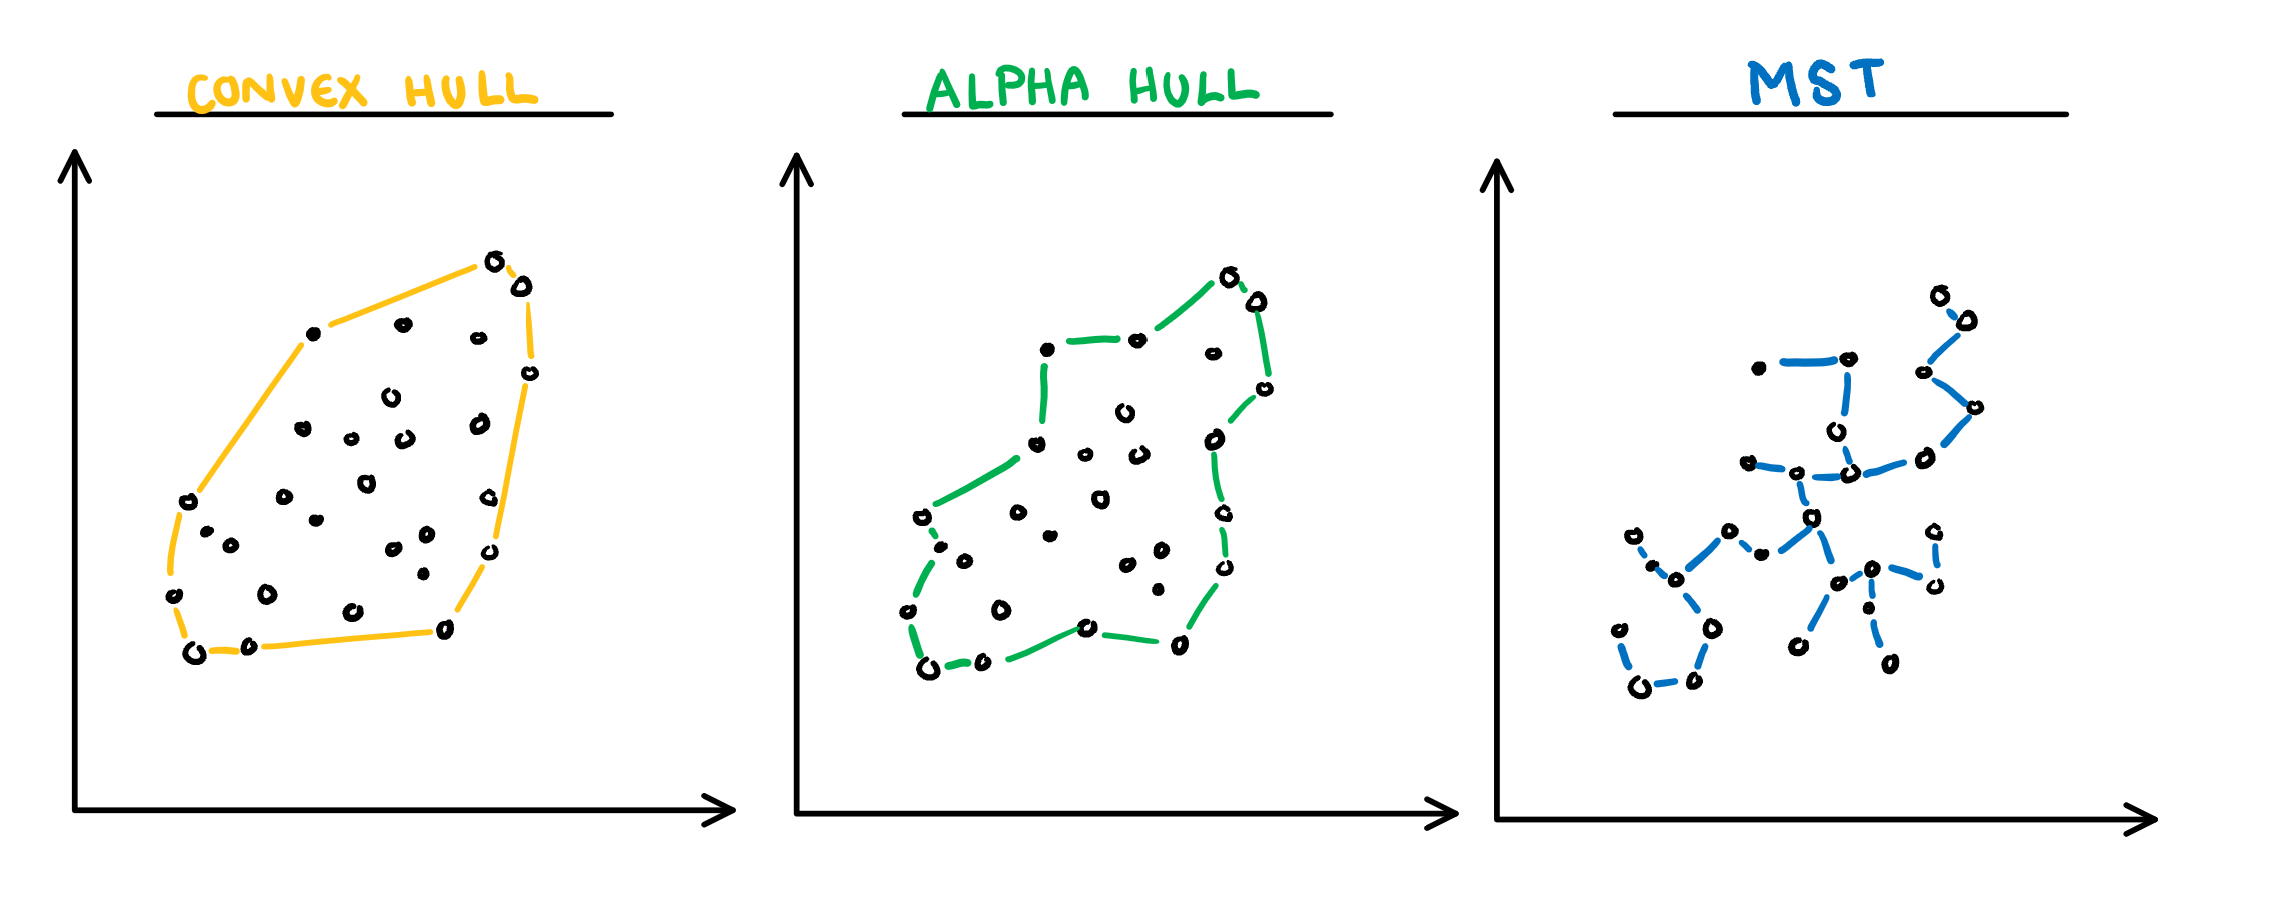
\includegraphics[width=1\linewidth,height=0.3\textheight]{figures/draw1} \caption[The building blocks for graph-based scagnostics]{The building blocks for graph-based scagnostics}(\#fig:building-blocks)
\end{figure}
\end{Schunk}

\hypertarget{graph-based-scagnostics}{%
\subsection{Graph-based scagnostics}\label{graph-based-scagnostics}}

The nine scagnostics defined in \emph{Scagnostic Distributions} are
detailed below with an explanation, formula, and visualisation. We will
let \emph{A}= alpha Hull \emph{C}= convex hull, \emph{M} = minimum
spanning tree, and \emph{s}= the scagnostic measure. Since some of the
measures have some sample size dependence, we will let \emph{w} be a
constant that adjusts for that.

\begin{itemize}
\tightlist
\item
  \textbf{Convex:} Measure of how convex the shape of the data is.
  Computed as the ratio between the area of the alpha hull (A) and
  convex hull (C).
\end{itemize}

\[s_{convex}=w\frac{area(A)}{area(C)}\]


\includegraphics{figures/drawconvex.png}

\begin{itemize}
\tightlist
\item
  \textbf{Skinny:} A measure of how ``thin'' the shape of the data is.
  It is calculated as the ratio between the area and perimeter of the
  alpha hull (A) with some normalisation such that 0 correspond to a
  perfect circle and values close to 1 indicate a skinny polygon.
\end{itemize}

\[s_{skinny}= 1-\frac{\sqrt{4\pi area(A)}}{perimeter(A)}\]


\includegraphics{figures/drawskinny.png}

\begin{itemize}
\tightlist
\item
  \textbf{Outlying:} A measure of proportion and severity of outliers in
  dataset. Calculated by comparing the edge lengths of the outlying
  points in the MST with the length of the entire MST.
\end{itemize}

\[s_{outlying}=\frac{length(M_{outliers})}{length(M)}\]


\includegraphics{figures/drawoutlying.png}

\begin{itemize}
\tightlist
\item
  \textbf{Stringy:} This measure identifies a ``stringy'' shape with no
  branches, such as a thin line of data. It is calculated by comparing
  the number of vertices of degree two (\(V^{(2)}\)) with the total
  number of vertices (\(V\)), dropping those of degree one
  (\(V^{(1)}\)).
\end{itemize}

\[s_{stringy} = \frac{|V^{(2)}|}{|V|-|V^{(1)}|}\]

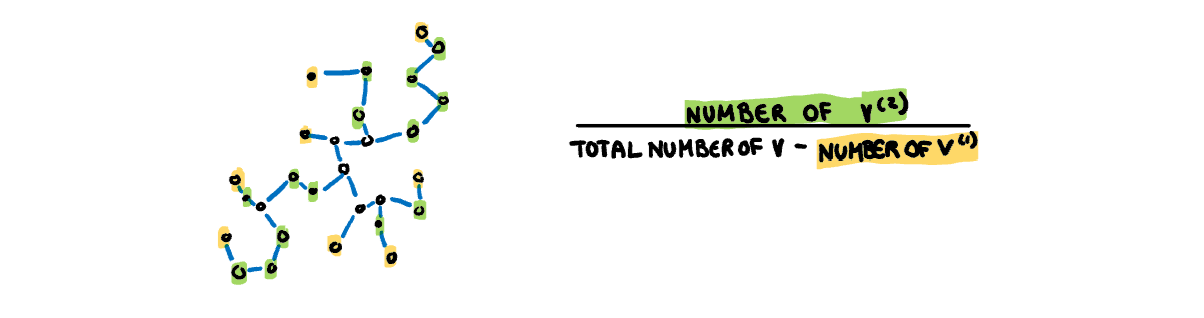
\includegraphics{figures/drawstringy.png}

\begin{itemize}
\tightlist
\item
  \textbf{Skewed:} A measure of skewness in the edge lengths of the MST
  (not in the distribution of the data). It is calculated as the ratio
  between the 40\% IQR and the 80\% IQR, adjusted for sample size
  dependence.
\end{itemize}

\[s_{skewed} = 1-w(1-\frac{q_{90}-{q_{50}}}{q_{90}-q_{10}})\]

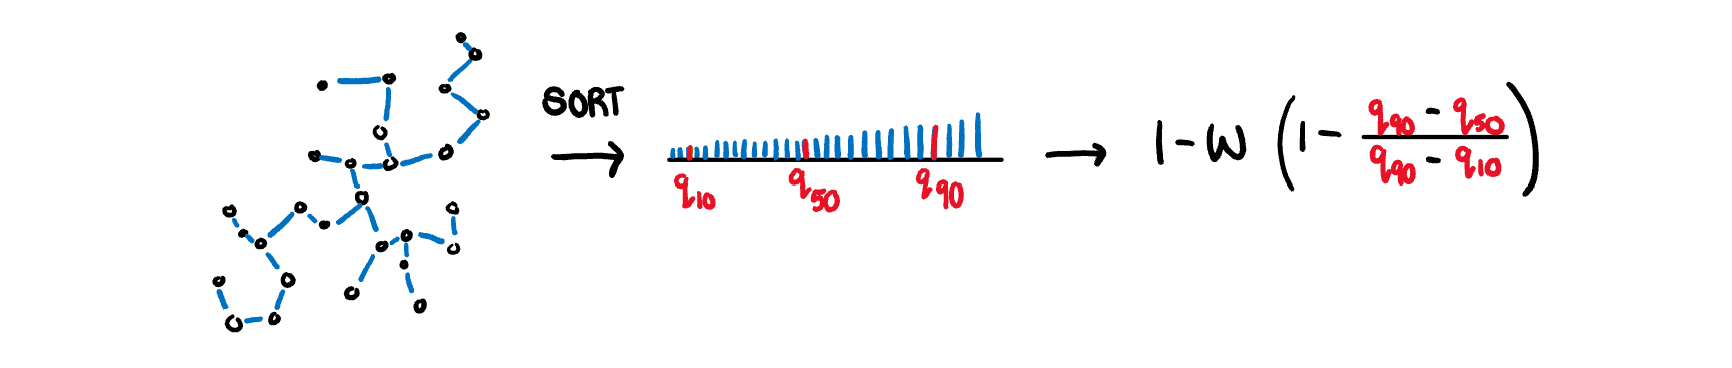
\includegraphics{figures/drawskewed.png}

\begin{itemize}
\tightlist
\item
  \textbf{Sparse:} Identifies if the data is sporadically located on the
  plane. Calculated as the 90th percentile of MST edge lengths.
\end{itemize}

\[s_{sparse}= wq_{90}\]

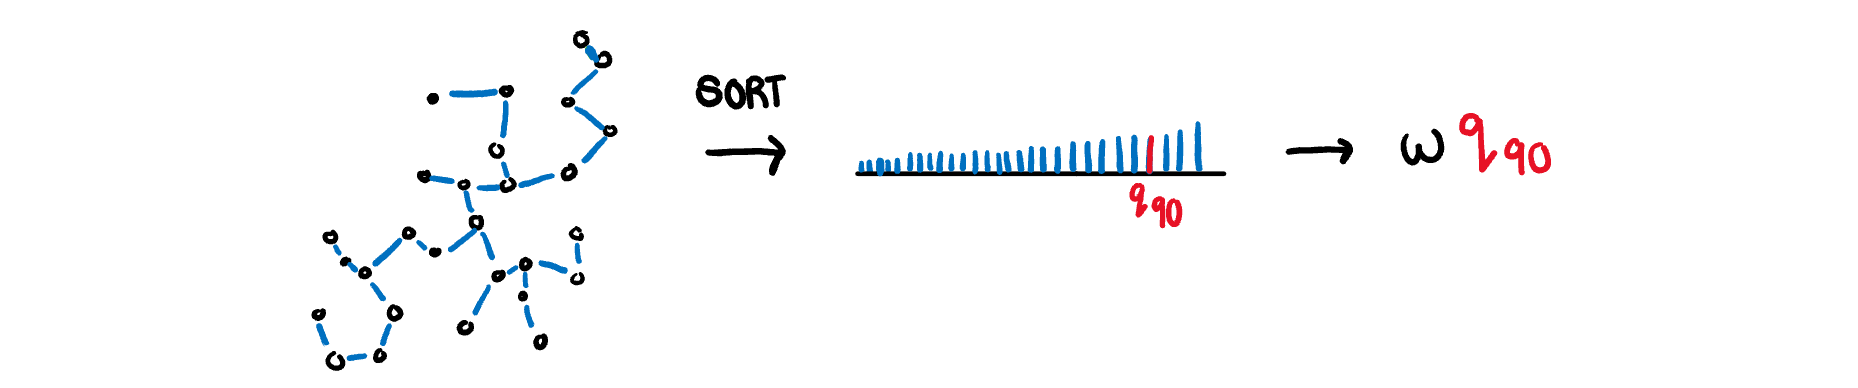
\includegraphics{figures/drawsparse.png}

\begin{itemize}
\tightlist
\item
  \textbf{Clumpy:} This measure is used to detect clustering and is
  calculated through an iterative process. First an edge J is selected
  and removed from the MST. From the two spanning trees that are created
  by this break, we select the largest edge from the smaller tree (K).
  The length of this edge (K) is compared to the removed edge (J) giving
  a clumpy measure for this edge. This process is repeated for every
  edge in the MST and the final clumpy measure is the maximum of this
  value over all edges.
\end{itemize}

\[\max_{j}[1-\frac{\max_{k}[length(e_k)]}{length(e_j)}]\]\\
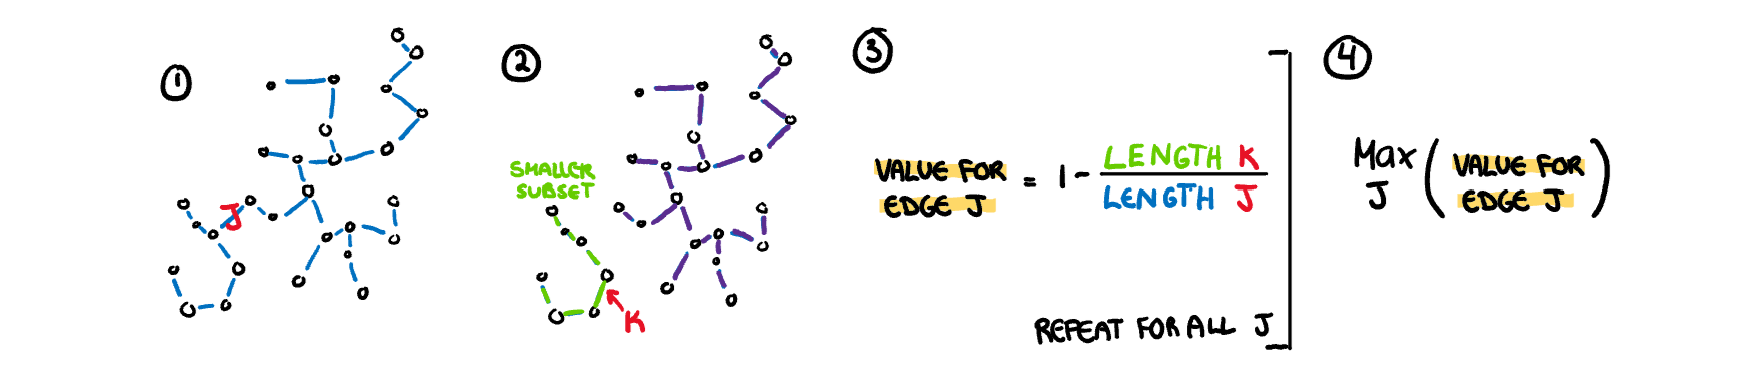
\includegraphics{figures/drawclumpy.png}

\begin{itemize}
\tightlist
\item
  \textbf{Striated:} This measure identifies features such as
  discreteness by finding parallel lines, or smooth algebraic functions.
  Calculated by counting the proportion of acute (0 to 40 degree) angles
  between the adjacent edges of vertices with only two edges.
\end{itemize}

\[\frac1{|V|}\sum_{v \in V^{2}}I(cos\theta_{e(v,a)e(v,b)}<-0.75)\]\\
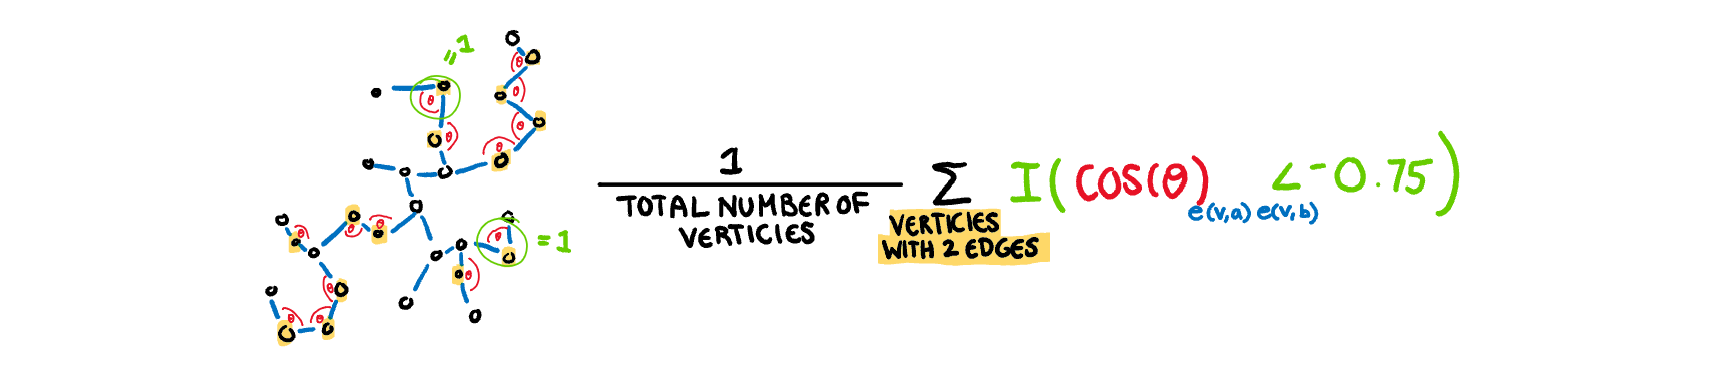
\includegraphics{figures/drawstriated.png}

\begin{itemize}
\tightlist
\item
  \textbf{Monotonic:} Checks if the data has an increasing or decreasing
  trend. Calculated as the Spearman correlation coefficient, i.e.~the
  Pearson correlation between the ranks of x and y.
\end{itemize}

\[s_{monotonic} = r^2_{spearman}\]
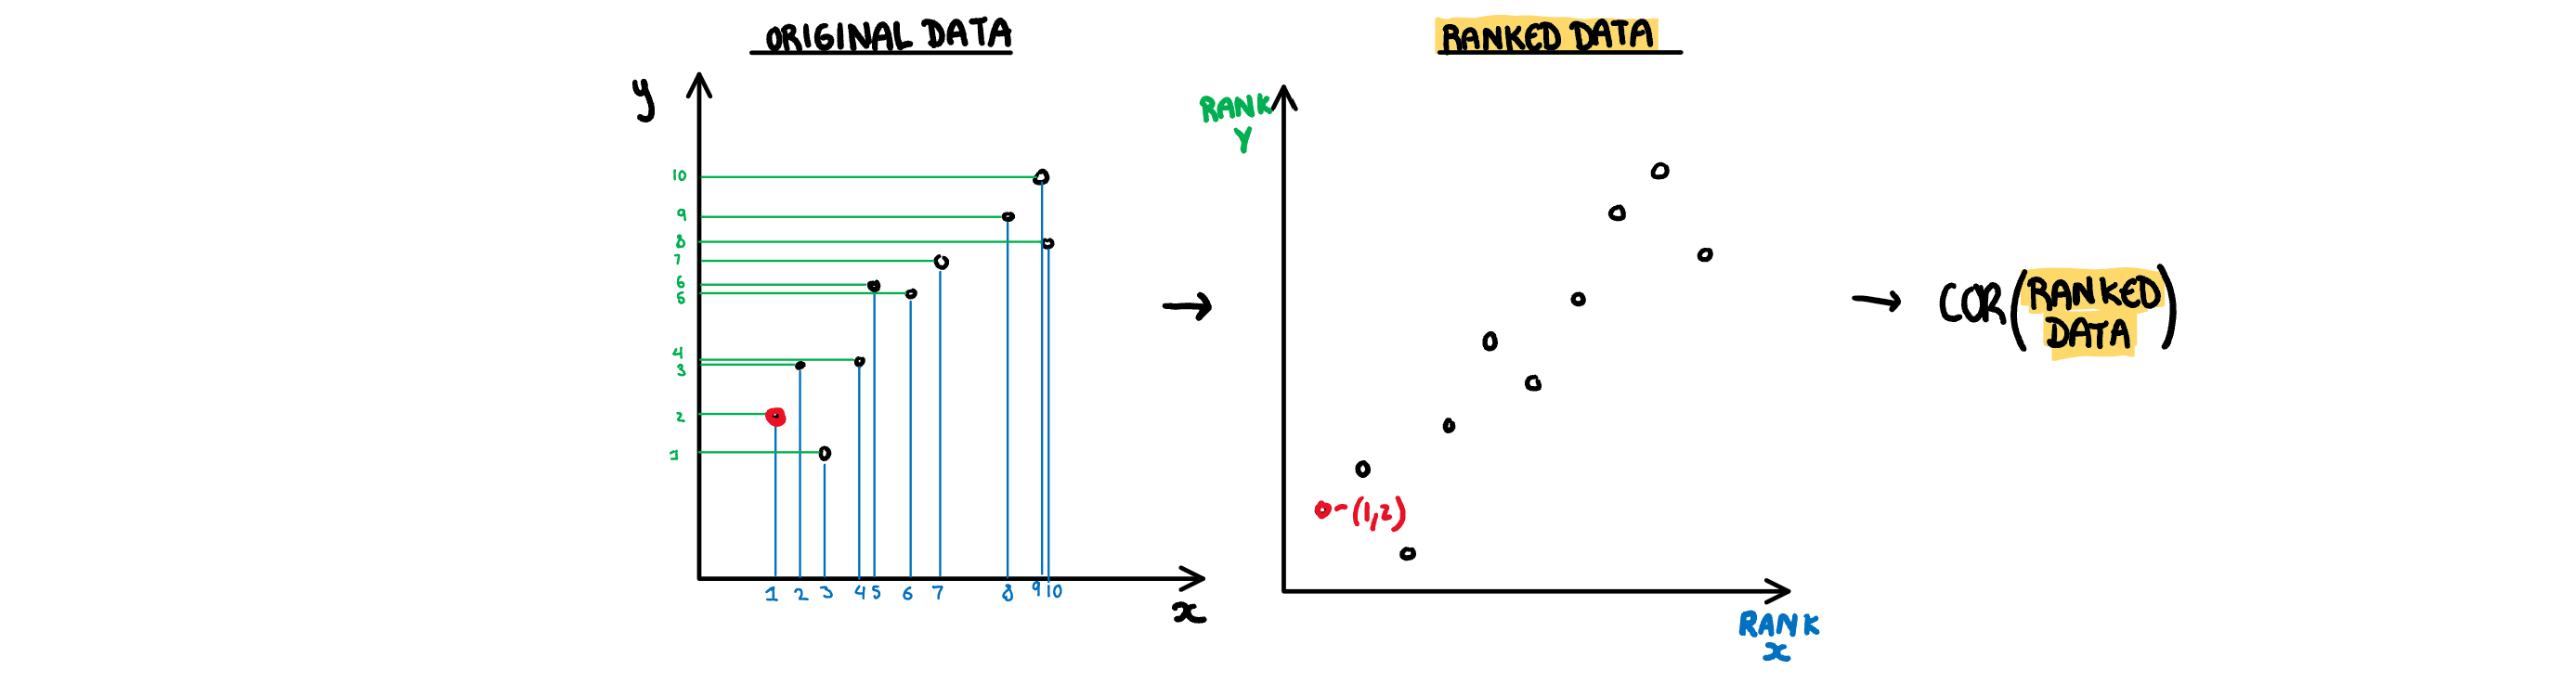
\includegraphics{figures/drawmonotonic.png}

\hypertarget{association-based-scagnostics}{%
\subsection{Association-based
scagnostics}\label{association-based-scagnostics}}

The two additional scagnostics discussed by Katrin Grimm are described
below.

\begin{itemize}
\tightlist
\item
  \textbf{Splines:} Measures the functional non-linear dependence by
  fitting a penalised splines model on X using Y, and on Y using X. The
  variance of the residuals are scaled down by the axis so they are
  comparable, and finally the maximum is taken. Therefore the value will
  be closer to 1 if either relationship can be decently explained by a
  splines model.
\end{itemize}

\[s_{splines}=\max_{i\in x,y}[1-\frac{Var(Residuals_{model~i=.})}{Var(i)}]\]

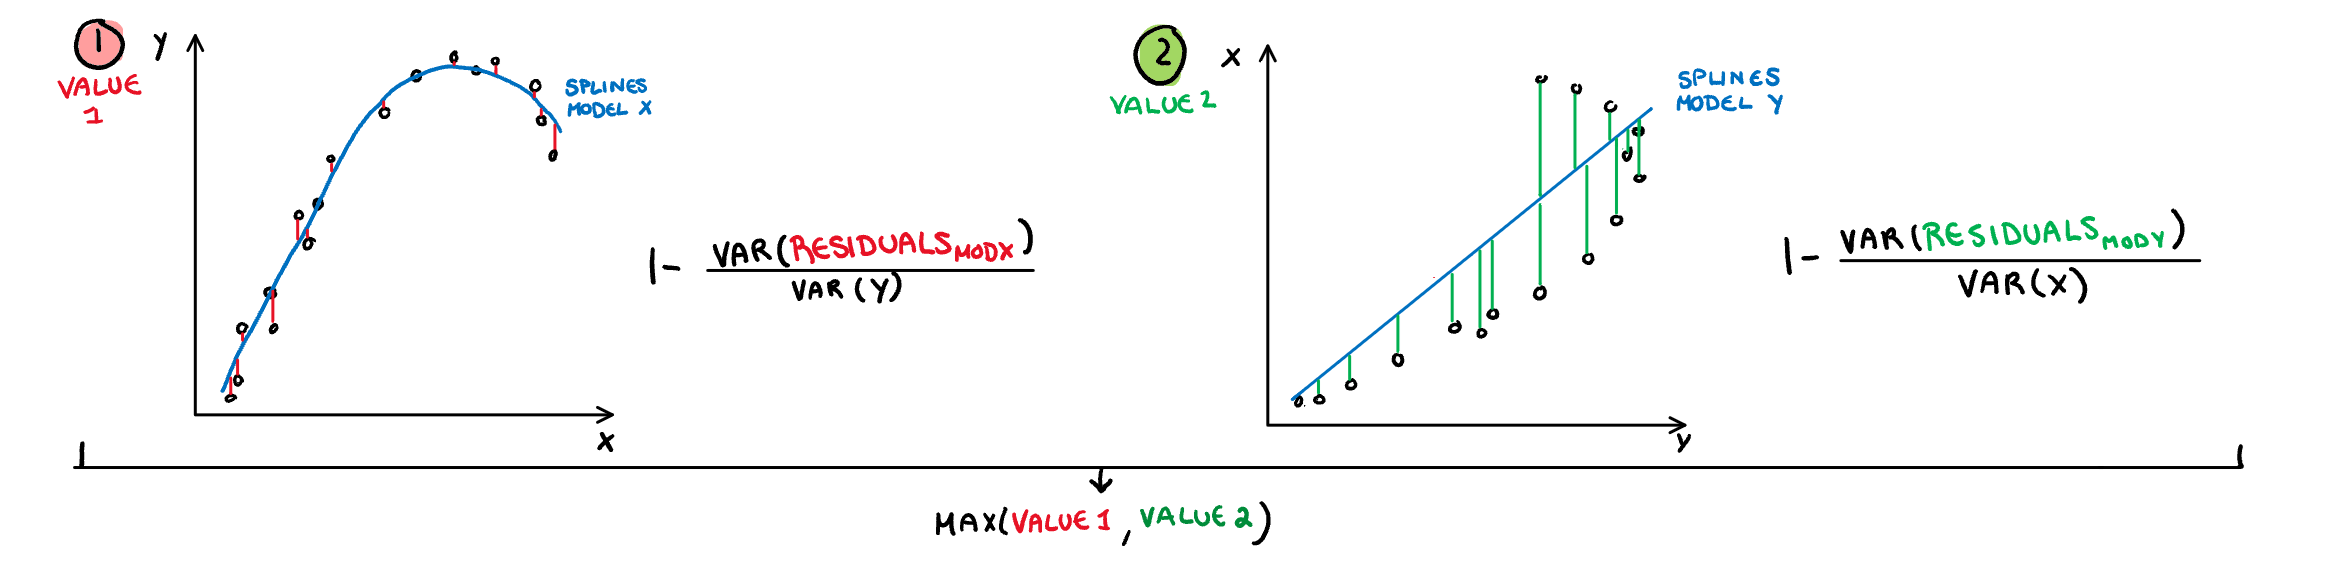
\includegraphics{figures/drawsplines.png}

\begin{itemize}
\tightlist
\item
  \textbf{Dcor:} A measure of non-linear dependence which is 0 if and
  only if the two variables are independent. Computed using an ANOVA
  like calculation on the pairwise distances between observations.
\end{itemize}

\[s_{dcor}= \sqrt{\frac{\mathcal{V}(X,Y)}{\mathcal{V}(X,X)\mathcal{V}(Y,Y)}}\]\\
where \[\mathcal{V}
(X,Y)=\frac{1}{n^2}\sum_{k=1}^n\sum_{l=1}^nA_{kl}B_{kl}\]\\
where \[A_{kl}=a_{kl}-\bar{a}_{k.}-\bar{a}_{.j}-\bar{a}_{..}\]
\[B_{kl}=b_{kl}-\bar{b}_{k.}-\bar{b}_{.j}-\bar{b}_{..}\]

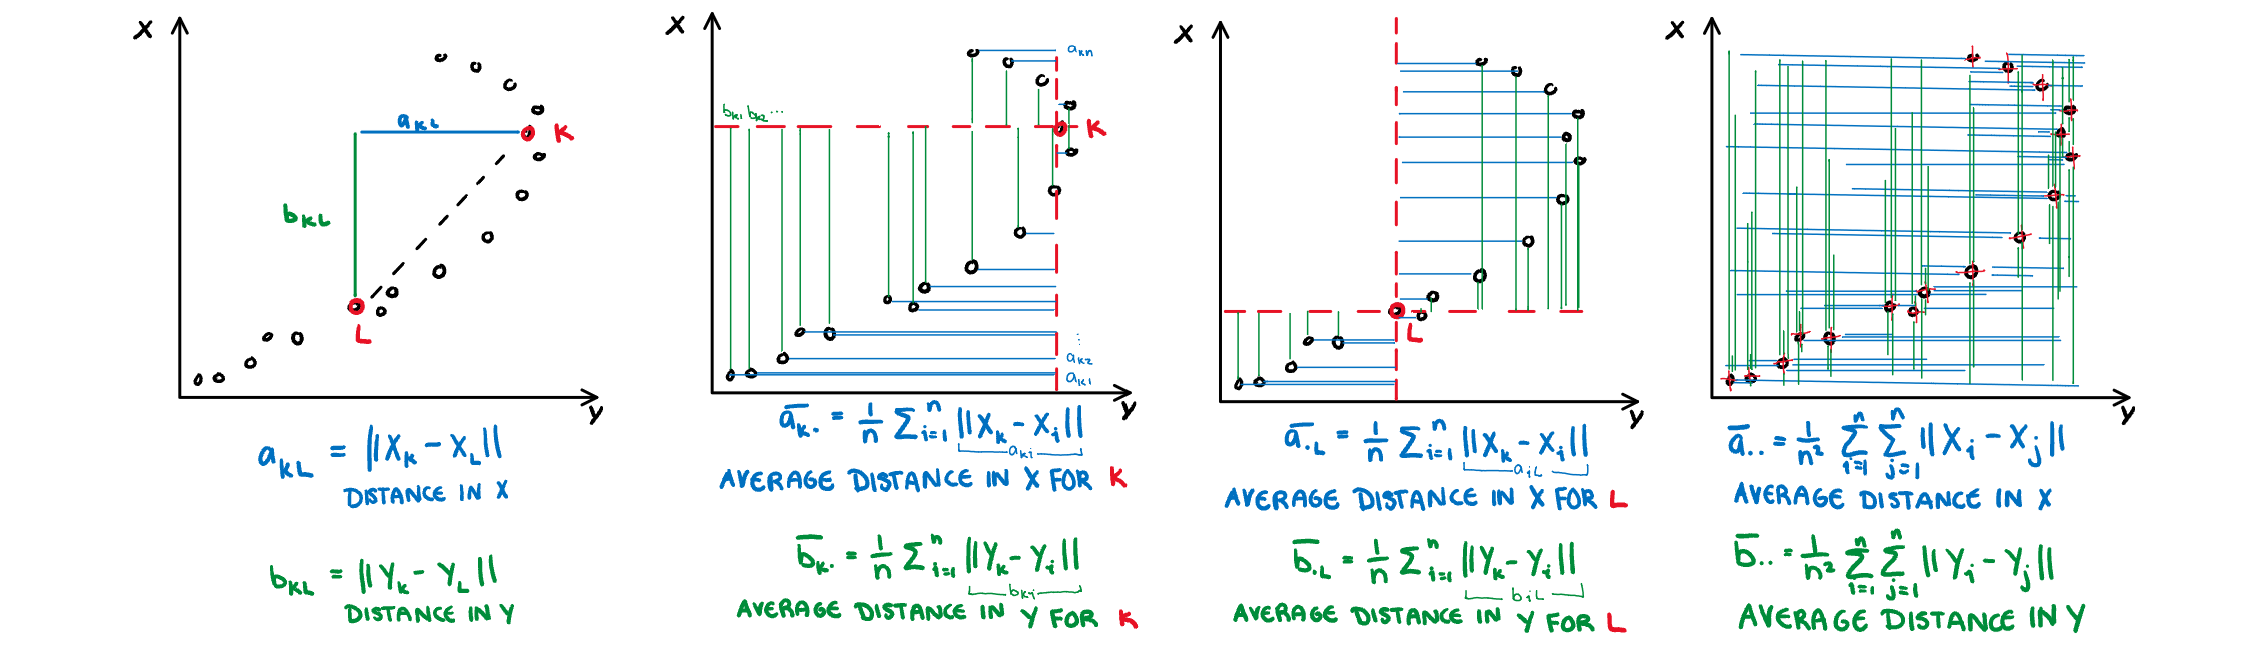
\includegraphics{figures/drawdcor.png}

\hypertarget{checking-the-scagnostics-calculations}{%
\subsection{Checking the scagnostics
calculations}\label{checking-the-scagnostics-calculations}}

Maybe use Anscombe and datasaurus and the features data here

\hypertarget{software-implementation}{%
\section{Software implementation}\label{software-implementation}}

\hypertarget{installation}{%
\subsection{Installation}\label{installation}}

\hypertarget{functions}{%
\subsection{Functions}\label{functions}}

\hypertarget{tests}{%
\subsection{Tests}\label{tests}}

\hypertarget{examples}{%
\section{Examples}\label{examples}}

\hypertarget{collections-of-time-series}{%
\subsection{Collections of time
series}\label{collections-of-time-series}}

A paragraph describing the compenginets data

\begin{Schunk}

\includegraphics[width=1\linewidth]{mason-lee-laa-cook_files/figure-latex/scatmatstatic-1} \end{Schunk}

\hypertarget{parkinsons}{%
\subsection{Parkinsons}\label{parkinsons}}

\hypertarget{black-holes-and-netron-star-mergers}{%
\subsection{Black holes and netron star
mergers?}\label{black-holes-and-netron-star-mergers}}

\hypertarget{summary}{%
\subsection{Summary}\label{summary}}

\begin{verbatim}
\end{verbatim}

\bibliography{mason-lee-laa-cook.bib}

\address{%
Harriet Mason\\
Monash University\\%
Department of Econometrics and Business Statistics\\ Melbourne,
Australia\\
%
\url{https://www.britannica.com/animal/quokka}\\%
\textit{ORCiD: \href{https://orcid.org/0000-1721-1511-1101}{0000-1721-1511-1101}}\\%
\href{mailto:hmas0003@student.monash.edu}{\nolinkurl{hmas0003@student.monash.edu}}%
}

\address{%
Stuart Lee\\
Genentech\\%
\\
%
\url{https://stuartlee.org}\\%
\textit{ORCiD: \href{https://orcid.org/0000-0003-1179-8436}{0000-0003-1179-8436}}\\%
\href{mailto:stuart.andrew.lee@gmail.com}{\nolinkurl{stuart.andrew.lee@gmail.com}}%
}

\address{%
Ursula Laa\\
University of Natural Resources and Life Sciences\\%
Institute of Statistics\\ Vienna, Austria\\
%
\url{https://uschilaa.github.io}\\%
\textit{ORCiD: \href{https://orcid.org/0000-0002-0249-6439}{0000-0002-0249-6439}}\\%
\href{mailto:ursula.laa@boku.ac.at}{\nolinkurl{ursula.laa@boku.ac.at}}%
}

\address{%
Dianne Cook\\
Monash University\\%
Department of Econometrics and Business Statistics\\ Melbourne,
Australia\\
%
\url{https://dicook.org}\\%
\textit{ORCiD: \href{https://orcid.org/000-0002-3813-7155}{000-0002-3813-7155}}\\%
\href{mailto:dicook@monash.edu}{\nolinkurl{dicook@monash.edu}}%
}
